\documentclass[12pt, a4paper]{article}


\usepackage[centertags]{amsmath}
\usepackage{amsfonts,amssymb,amsthm}
\usepackage{graphicx}
\usepackage{tabularx}
\usepackage[a4paper, total={6in, 8in}]{geometry}
\usepackage{iitbcsresyn}
\usepackage{setspace}
\usepackage{textcomp}
\usepackage{epstopdf}
\usepackage{setspace}
\usepackage{sectsty}
\usepackage[font=small,format=hang,labelfont=bf]{caption}
\usepackage[font=small]{subcaption}
%\usepackage{rotating}

\usepackage{bm}

\usepackage{breqn}
\usepackage{siunitx}
\renewcommand{\baselinestretch}{1.2} %line spacing
%\chapterfont{\vspace{25mm}\centering}
%\textwidth 6in
% Title Page

%paragraph space
\usepackage{parskip}

\usepackage{mdwlist}
\usepackage{paralist}

\usepackage{breqn}


\usepackage{etoolbox}

\usepackage{pifont}
\usepackage{charter} %bookman
%last import
\usepackage{hyperref}

\begin{document}

\pagenumbering{arabic}
\pagestyle{plain}
\def\title{Development of Auto-Encoder Based Methods for Synthetic Aperture Radar Image Analysis}
\def\degree{Doctor of Philosophy}
\def\who{Shaunak De (134316001)}
\def\guide{Prof. Avik Bhattacharya}
\def\when{15 February 2018}

\coverpage

% % % % %
\section{Introduction}

Remotely sensed images acquired by space-borne or airborne sensors have revolutionized earth observation allowing an unprecedented ability to image and observe large areas of the planet's surface with high temporal repetitivity. This has opened new avenues for the monitoring of dynamic earth processes. Long-term earth observation missions have ensured data continuity over decades allowing the characterization of natural and anthropocentric processes and changes. However, in order for the images to be used for these applications, they must be processed so that the information of interest is brought out. 

Classification of remote sensing data involves grouping of pixels into homogeneous groups, usually representing a type of land cover. This allows the generation of thematic maps. Traditionally thematic maps have been produced by a field survey of the region to be mapped, or by manual analysis of data. 
Many of these maps, especially those used for disaster management or the tracking of fast-changing geo-dynamics, must be generated rapidly with a fair degree of accuracy. 
The all-weather, day-night imaging capability of a Synthetic Aperture Radar (SAR) system is highly desirable for defense, security and monitoring applications, where time-critical imaging is required. Unmanned aerial vehicle (UAV) borne SAR systems are being operationally used for information gathering. A peripatetic platform like this is capable of high repetivity and frequent re-visits. Thus it generates a high volume of data. 
%
In such a scenario, the ability to extract information from the datasets in an automated manner is important. However, object recognition and classification in SAR images is not without its challenges. SAR images suffer from geometric distortions and speckle-like noise patterns which are inherent to the process of SAR image formation. Polarimetric SAR (PolSAR) images contain more information than single or dual channel SAR, but it is important to develop techniques to fully utilize this information.  

Automation in classification and identification tasks, or at least part-automation, can helpfully utilize the potential of the large data volumes. Machine learning algorithms can help collate information from the data, which can eventually lead to the extraction of knowledge from the information. Learning machines are designed to tune their internal parameters according to the input data to improve their efficiency and/or accuracy. Machine learning algorithms are able to utilize the extensive data quantities. However, traditional machine learning algorithms usually need specially designed input features, either from $a-priori$ information about the distribution of the data, or domain knowledge, for a particular application, making complete automation prohibitive. Also, beyond a point, increase in the amount of available training data does not lead to a corresponding improvement in task efficacy.

Deep Learning is a new approach based on the workings of the human cognitive system pioneered in 2006~\cite{goodfellow2016deep}. The principle behind deep learning is to distribute a complex task into simpler subtasks. Different parts of the network can then be responsible for each sub-task, eventually being connected cohesively to solve the original task. It has shown superior performance as compared to 'shallow' approaches in various classification and recognition challenges and is rapidly being applied to diverse fields like image classification, object recognition, speech and language processing, etc. Deed learning techniques greatly benefit from increased training information, more so than other contemporary methods, making them a good fit for remote sensing applications in which high volumes of similar data is collected.  

A sub-set of deep learning techniques are auto-encoders, which are able to summarize the information content of the presented data in either a compressed, or sparse representation, to be operated on by a subsequent learning algorithm for improved task performance. However, the availability of labeled training information in the domain of remote sensing is limited. This thesis develops a set of novel methodologies that incorporate physical scattering principles into a Deep Neural Network architecture, especially auto-encoders, for he analysis of radar remote sensing images, in an effort to reduce the demand of training data and build models more in tune with the laws of our physical world.




\section{Motivation}

Optical remote sensing has been primarily used for earth observation, monitoring and disaster management applications. However, being a passive sensor, it's limited to operating in the presence of solar irradiation. Further, it is impeded by the presence of cloud cover. SAR, on the other hand, is an active imaging technique and has an advantage that it is able to operate independently of ambient illumination. It is also insensitive to the weather due to its capability of penetrating cloud cover. SAR is sensitive to both the wavelength scale geometrical and dielectric properties of the target, allowing it to ascertain information about the target that is not possible with reflectance alone. PolSAR is an advancement over SAR imaging, which uses a combination of transmit and receive polarizations in quadrature. Thus, it is sensitive to the wavelength-scale structure of the target and has better discrimination potential. To be able to exploit this increased target information fully, and to efficiently handle the increasing volume of data being collected by present and planned satellite constellations, automated analysis techniques must be developed. Machine learning algorithms are a reasonable choice for this task. However, hand-crafted features need to be designed from domain knowledge and require expert intervention, making it time-consuming and prohibitive for large data volumes. Deep learning aims to develop a simple feature representation internally and automatically without the need for hand-crafted or a specially designed input space. This makes deep learning techniques, like auto-encoders especially synergistic for PolSAR applications. The motivation for this thesis has been to explore the possibilities of enhancing Earth observation applications of PolSAR data using novel auto-encoder networks.

\section{Research Objectives}
In this thesis, novel deep learning algorithms and architectures centered around auto-encoder networks are proposed for various earth observation applications using fully polarimetric SAR data.
The methodologies have been developed and verified using airborne L-band UAVSAR, airborne C-, L-, P-band AIRSAR, spaceborne C-band RADARSAT-2 and spaceborne L-band ALOS-2 datasets. Applications have been demonstrated in the field of agricultural monitoring, urban classification, change detection and disaster response, 

The following objectives have been accomplished in the course of this thesis:

\begin{enumerate}
\item Auto-encoders have been demonstrated in finding an efficient sparse feature-space representation of PolSAR data.
\item Scattering physics has been incorporated in an auto-encoders architecture using a novel technique for data-augmentation, which improves generalization capacity. 
\item A novel deep-learning framework has been developed that outperformed state of the art techniques in the classification of urban areas, especially those not perpendicular to the line of sight of the radar.
\item Development of a novel semi-supervised technique that allows change detection in urban areas with very few training points using a region growing technique in the auto-encoder's feature space. 
\item A novel tensorization technique in conjunction with a spatial auto-encoder has been proposed that is able to combine information from multi-frequency bands to improve classification of natural areas.
\end{enumerate}


\section{Supervised Urban Classification }
The classification of urban areas in PolSAR data-sets is especially challenging, because of the problems related to orientation of targets with respect to the radar line of sight. When targets that exhibit even bounce scattering are oriented away from the radar line of sight, the co-polarized return is reflected away from the sensor, while the cross-polarized return level remains the same.

This makes such areas hard to distinguish from natural targets like forest and vegetation. This represents a major challenge for the classification algorithm\cite{hirose2006complex}. In general, polarization orientation angle shifts are observed in polatimetric SAR data which are induced by terrain slopes and complex scattering in urban
areas~\cite{yamaguchi2011four}. In turn, polarization orientation angle shifts can be induced by appropriate Euler rotations to form synthetic targets. They can be suitably leveraged for better generalization in machine learning algorithms. The process is used to generate a database containing simulated urban targets. The synthetic urban target database is used to train and extract features from a sparse stacked auto-encoder. 

Thus, the information about the targets and rotation is accounted for in the classification scheme, which helps to discriminate rotated urban areas without requiring explicit representation in the training stage. The advantage of using a deep learning based scheme is that, the network can be trained incrementally on a large volume of data, and subsequently used as a generalization for unseen data. This leads to a computationally efficient and fast classification phase. Given the commercial interests in deep learning at large scale, several GPU based specialized peripherals have been developed. These can be used to further speed up calculations and drastically reduce the training time over CPU bound computation.

The proposed approach for pixel classification of PolSAR data is shown in Figure~\ref{fig:0}. The first stage deals with the pre-processing of the PolSAR data and the generation of a generalized synthetic urban target database by transforming the input data to obtain a more general representation of the target. The second stage is an unsupervised feature learning step, which automatically learns an optimal representation of the generalized database using a stacked auto-encoder network. Finally, the third stage extracts optimal features from the previous stages, along with some statistical parameters and performs a supervised classification by using a multi-layer perceptron network.

\begin{figure}
\centering
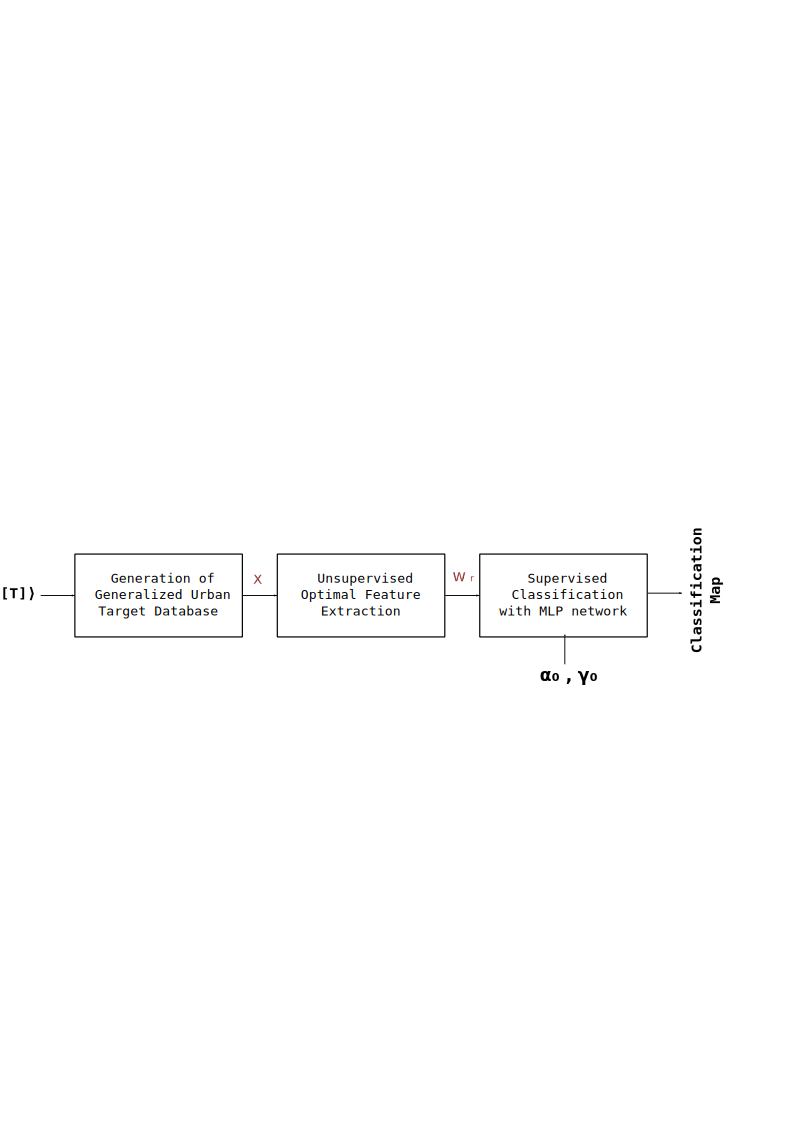
\includegraphics[width = 0.75\textwidth]{Figures/Method0}
\caption{Overview of the proposed supervised urban classification technique.}
\label{fig:0}
\end{figure}

The modular architecture allows for easy optimization of the hyper-parameters. The synthetic target database is created and classification performance is evaluated on an L-band airborne UAVSAR dataset and L-Band space-borne ALOS-2 dataset acquired over San Francisco, USA. The proposed technique shows an overall accuracy of $91.3\%$. An improvement over state of the art techniques is achieved, especially in urban areas rotated away from the radar line of sight. A representative set of results from depicting the proposed technique, in comparison to other state of the art techniques is shown in Figure~\ref{fig:comparison_al2}. 

\begin{figure}
\centering	
	\begin{subfigure}[t]{0.15\textwidth}
		\includegraphics[trim={150px 80px 40px 50px},clip,width=\columnwidth]{Figures/ALOS2_SF_3Class/OP_300} 
		\caption{Proposed}
		\label{fig:proposed_al2}
	\end{subfigure}
	~
	\begin{subfigure}[t]{0.15\textwidth}
		\includegraphics[trim={150px 80px 40px 50px},clip,width=\columnwidth]{Figures/ALOS2_SF_3Class/svm_classification_file_2016_04_07_12_23_47_rbf} 
		\caption{SVM RBF}
		\label{fig:al2_svm_rbf}
	\end{subfigure}
	~
	\begin{subfigure}[t]{0.15\textwidth}
		\includegraphics[trim={150px 80px 40px 50px},clip,width=\columnwidth]{Figures/ALOS2_SF_3Class/svm_classification_file_2016_04_07_12_20_26_lin} 
		\caption{SVM Polynomial}
		\label{fig:al2_svm_poly}
	\end{subfigure}
	~
	\begin{subfigure}[t]{0.15\textwidth}
		\includegraphics[trim={150px 80px 40px 50px},clip,width=\columnwidth]{Figures/ALOS2_SF_3Class/wishart_supervised_class_1x1_poc} 
		\caption{Wishart with POC}
		\label{fig:al2_wish_1_poc}
	\end{subfigure}
	~
	\begin{subfigure}[t]{0.15\textwidth}
		\includegraphics[trim={150px 80px 40px 50px},clip,width=\columnwidth]{Figures/ALOS2_SF_3Class/wishart_supervised_class_1x1} 
		\caption{Wishart}
		\label{fig:al2_wish_1}
	\end{subfigure}
	\caption{Comparison of common classification techniques with the proposed method.}
	\label{fig:comparison_al2}
\end{figure}



\section{Semi-Supervised Urban Classification }

The active imaging capabilities of a SAR system allows imaging in inclement weather and illumination conditions. This is highly desirable for urban mapping and change detection applications, especially in the tropical regions where the monsoons obscure urban centers from view of optical sensors for many months. It is also during this period that calamities like floods are most likely
to occur making the rapid imaging ability of SAR sensors crucial.
%
Change detection aims at identifying changes occurred on the ground between two or more acquisitions on the same geographical area at different time instants. The complexity of collecting ground reference samples makes unsupervised and semi-supervised approaches the most relevant in the field.
%
The approach proposed in this thesis takes an input, a pair of  images and learns a representation that maximizes the separation of changed areas from unchanged ones in the multi-temporal stacked feature vectors (manifold) domain. This representation is exploited by a weakly supervised neural network technique to generate a change map. The framework takes multi-temporal polarimetric SAR images as input and produces an output with 3 classes: changed urban areas, unchanged urban and unchanged natural areas. This kind of maps are useful for urban monitoring and rescue operations.

The block scheme of the proposed methodology is shown in Figure~\ref{fig:1}. Two PolSAR images acquired over the same geographic area at time instants $t_0$ and $t_1$ , are pre-processed and normalized before being given as input to a stacked auto-encoder network. The auto-encoder is trained in an unsupervised manner to create an optimal representation, assuming that only a very small amount of ground truth is available, a label aggregation step is undertaken before classification by a multi-layer perceptorn.

Ground reference labels are assumed to be available for only a small portion of the scene. This is a realistic assumption for disaster relief or monitoring efforts, where information would be available at a point of the scene where administrative efforts are concentrated. However the total number of labeled pixels is l << N and hence the framework is said to be weakly supervised. The use of very few samples will lead to poor accuracies as the dataset is under-represented. Thus a label aggregation step is performed. In the representational space a convex-hull is fitted for each class on the labeled samples, in order to reduce the number of considered points and simplify computation. Then a minimum volume bounding ellipsoid is fitted on these points. Thinning along the radial axis of the ellipsoid is performed to exclude points that lie on the periphery of the volume, having a lower probability of belonging to the class than a more internal point. After thinning, points that lie within each ellipsoid are assumed to belong to the corresponding class and are preselected for labeling. From these, an equal number of samples $L$ are chosen per-class using the reservoir sampling technique to preserve the distribution of each class.  These samples are then to assigned the corresponding class labels, increasing the number of labeled samples available to the final classifier. A multi-layer perceptron network is used to perform the final classification with the aggregated labels. The extracted representation $z$ is used in the classification with the aggregated labels to produce the final output map.

Effectiveness of the technique is demonstrated on a L-band UAVSAR dataset acquired over Los Angeles, California with a resolution of 0.4m in azimuth and 1.66m in range. The study-area is a dense urban
area with changes occurring primarily due to the effects of urbanization. The objective of the proposed methodology is to characterize the construction and destruction of urban areas, while simultaneously classifying unchanged urban and natural areas in the rest of the scene. Qualitatively and Quantitatively, the output corresponds well with the changed areas observed in the Pauli composition image pair and has low misclassification. The overall accuracy is $92.35\%$ with $\kappa=0.88$. 



\begin{figure}
\centering
\includegraphics[width = 0.65\textwidth]{Figures/BLOCK}
\caption{Overview of the proposed semi-supervised urban change detection technique.}
\label{fig:1}
\end{figure}

\section{Multi-frequency Crop Classification}
The multi-frequency polarized waves are susceptible to different structure, orientation and dielectric
properties of the medium. Various PolSAR systems (viz. AIRSAR, EMISAR, and F-SAR) are capable of simultaneous multi-frequency full PolSAR data acquisition allowing for improved target characterization. The combination of multi-frequency information however causes a simultaneous increase in dimensionality of the feature set. In classical machine learning, an increase in dimensionality causes increased complexity for the learning technique. However, by exploiting techniques like the deep neural network, it is possible to incorporate the information without the dimensionality reduction step. Upcoming space-borne missions are planned to have multi-frequency systematic PolSAR data collection capabilities, making it important to develop frameworks capable of leveraging the data.
Efficient techniques for augmentation and fusion of the acquired data for the analysis of enhanced information content is desirable. The proposed tensorization framework allows for homogeneous composition of information from each frequency-band and prevents an \emph{a-priori} bias towards a dominant band. Hence, such a combination leads to a higher dimensional representation which, in general, is more separable for classification tasks if exploited by suitable learning algorithms~\cite{smolensky1990tensor}. 

\begin{figure}
	\centering
	\includegraphics[width=0.7\textwidth]{Figures/AE}
	\caption{Schematic diagram of the proposed framework.}
	\label{fig:ANN}
\end{figure}


The methodology is divided into two components: Synthesis of the feature vector using tensorization and classification using an deep neural network.

Two multi-frequency PolSAR datasets from the AIRSAR system are used in this study. A C-, L-, P-band dataset  acquired over and agricultural area in Flevoland, Netherlands on 3 July 1991, and a C-, L-band dataset acquired over a forested area in Landes, France on 20 June 1991.

The benefit of using the tensorization framework is demonstrated by comparing it  against the simple augmentation of all frequency bands. In the augmented case, the $1\times9$ resultant input vector is formed by appending individual frequency input vectors. The proposed framework is also compared with standard classification techniques like Support Vector Machine with a Radial Basis Function kernel (SVM-RBF) and Extreme Learning Machine.

In the Flevoland agricultural dataset, the crops present in the scene are Peas, Wheat, Rapeseed (R.Seed), Lucerne, Barley, Potato and Beet. Most of the crops are in the middle of their growth stage.  
It can be seen that the tensor combination of all three bands is the most informative and has the best classification performance with an overall accuracy of $98.23\%$ with $\kappa = 0.94$. In this combination, all classes are correctly identified with the potatoes and sugar beet having the least accuracies at $91.97\%$ and $89.82\%$, respectively.

The Landes site is a pine forest, with tree-patches of differing ages. A reference map is constructed from observation of polarimetric signatures. To establish the robustness of the results an experiment is conducted on the Landes dataset with two frequency bands. The classification results are presented. The tensorized pair $CL$ has an overall accuracy of $96.23\%$ with $\kappa=0.94$. This exceeds the classification performance obtained by simple augmentation ($CL_+$), which has an overall accuracy of $92.15\%$ with $\kappa=0.91$. For individual bands, the L-band, with an overall accuracy of  $89.73\%$ with $\kappa=0.70$, outperforms the C-band alone, which has an overall accuracy of  $77.42\%$ with $\kappa=0.62$. In this case, the greater penetration ability of L-band is crucial in being able to segregate the age of the trees, since return from the top foliage of the tree is nearly identical irrespective of their ages. A subset of the results are presented in Figure~\ref{fig:MultiFreq}.


\begin{figure}
\centering
        %~ %add desired spacing between images, e. g. ~, \quad, \qquad, \hfill etc. 
          %(or a blank line to force the subfigure onto a new line)
        \begin{subfigure}[b]{0.15\textwidth}
            \includegraphics[width=\textwidth]{Figures/Kron/CL_COLOUR}
            \caption{}
            \label{fig:CL}
        \end{subfigure}
        ~ %add desired spacing between images, e. g. ~, \quad, \qquad, \hfill etc. 
        %(or a blank line to force the subfigure onto a new line)
        \begin{subfigure}[b]{0.15\textwidth}
            \includegraphics[width=\textwidth]{Figures/Kron/CP_COLOUR}
            \caption{}
            \label{fig:CP}
        \end{subfigure}
        ~ %add desired spacing between images, e. g. ~, \quad, \qquad, \hfill etc. 
          %(or a blank line to force the subfigure onto a new line)
        \begin{subfigure}[b]{0.15\textwidth}
            \includegraphics[width=\textwidth]{Figures/Kron/LP_COLOUR}
            \caption{}
            \label{fig:LP}
        \end{subfigure}
            ~ %add desired spacing between images, e. g. ~, \quad, \qquad, \hfill etc. 
            %(or a blank line to force the subfigure onto a new line)
            \begin{subfigure}[b]{0.15\textwidth}
                \includegraphics[width=\textwidth]{Figures/Kron/CLP_COLOUR}
                \caption{}
                \label{fig:CLP}
            \end{subfigure}
        ~
        \begin{subfigure}[b]{0.15\textwidth}
            \includegraphics[width=\textwidth]{Figures/Kron/CLP2_COLOUR}
            \caption{}
            \label{fig:CLPaug}
        \end{subfigure}
        ~
        \begin{subfigure}[b]{0.15\textwidth}
                  \includegraphics[width=\textwidth]{Figures/Kron/SVM_COLOUR}
                  \caption{}
                  \label{fig:SVM}
        \end{subfigure}
        ~
        \begin{subfigure}[b]{0.15\textwidth}
                        \includegraphics[width=\textwidth]{Figures/Kron/ELM_COLOR}
                        \caption{}
                        \label{fig:ELM}
        \end{subfigure}
        
        \begin{tabular}{llllllll}
        \includegraphics[width=0.01\textwidth]{Figures/Kron/Legend/Pea} & Peas & \includegraphics[width=0.01\textwidth]{Figures/Kron/Legend/Wheat} & Wheat &  \includegraphics[width=0.01\textwidth]{Figures/Kron/Legend/Rseed} & R.Seed & \includegraphics[width=0.01\textwidth]{Figures/Kron/Legend/Luc} & Lucerne  \\
        \includegraphics[width=0.01\textwidth]{Figures/Kron/Legend/Barley} & Barley & \includegraphics[width=0.01\textwidth]{Figures/Kron/Legend/Potatoe} & Potato  & \includegraphics[width=0.01\textwidth]{Figures/Kron/Legend/Beet} & Beet &  & 
        \end{tabular}
    \caption{Classification outputs of input vectors derived from (a) $CL$ (b) $CP$ (c) $LP$ (d) $CPL$ (e) $CLP_{+}$ band combinations with the proposed method and using (f) SVM-RBF (g) ELM methods. The SVM-RBF and ELM methods do not inherently generate a confidence map and are presented unmasked.}\label{fig:MultiFreq}
\end{figure}

\section{Snow-Cover Mapping }

Snow cover variation is a sensitive indicator of environmental change. Therefore, snow cover mapping is a critical exercise which is supposed to be performed at regular intervals. Observations at periodic intervals require a sensor independent of time and weather. Microwave remote sensing is a reliable tool for the timely observation of spatial and temporal variability of snow-pack characteristics~\cite{cloude2010polarisation}. 

In this work, a snow cover mapping framework is proposed which uses the Poincar\'e sphere parameters obtained from the Radarsat-2 full-polarimetric SAR images. An unsupervised auto-encoder is used to learn an optimal representation of these parameters. This is followed by a feed forward network which generates the final snow-cover map as a two-class classification process.

The test site is located in the Manali-Dhundi region between the latitudes of $32^{o} 11^{'} N$ to $32^{o} 30^{'} N$, and between the longitudes of $77^{o} 2^{'} E$to $77^{o} 24^{'} E$. In this study a multi-spectral scene from Landsat-8 and a SAR data-set acquired by Radarsat-2 is used. The SAR scene was acquired on 18 March 2015 at 6:14 AM in the descending pass configuration with incidence angle in the range $46.0^\circ-47.2^\circ$ across the swath. The sensor was in the 'Standard Quad-Pol' yielding a $25\times25$ Km fully polarimetric measurement with HH, VV, HV and VH polarizations at a spatial resolution of 11.8m in range and 5.1m in azimuth.

\begin{figure}
\centering
\includegraphics[width=0.7\textwidth]{Figures/SnowCover2018/FlowChart}
\caption{Overall description of the Neural Network.}
\label{fig:flow}
\end{figure}

The neural network is comprised of two parts, an unsupervised auto-encoder for feature representation learning, and a supervised feed-forward network for supervised classification as shown in Fig.~\ref{fig:flow}. 
%
The auto-encoder has five layers: two encoding layers, two decoding layers and one representational layer, whose weights are denoted as $Z$. During training of the auto encoder, the feed forward network is disconnected i.e. weight updates for it are suspended. Rectified linear unit is used as the activation function to overcome the issue of vanishing gradients during training in a deep network. After the training phase of the auto-encoder, the representational layer is extracted by applying the Poincar\'e sphere parameters and saving the weights of $Z$, in a pixel-by-pixel fashion. These extracted weights are used as input for the feed forward network. 

The auto encoder is set up such that the dimensionality of $Z$ is greater than that of $X$. The FF network is a three layer fully connected supervised feed forward network. The extracted representation $Z$ is given as input along with training labels to the feed forward network. It is trained in a supervised manner with Sigmoid nodes used as non-linearities. The training in this case is governed by the $L2$ loss. After training, the unlabeled pixels are presented to the network, and the output response is monitored. The pixel is classified into the class corresponding to the node with the highest response. 

\begin{figure}
\centering
\begin{subfigure}[b]{0.35\columnwidth}
\includegraphics[width=\textwidth]{Figures/SnowCover2018/Hyb}
\caption{}
\end{subfigure}
~
\begin{subfigure}[b]{0.35\columnwidth}
\includegraphics[width=\textwidth]{Figures/SnowCover2018/Lin} 
\caption{}
\end{subfigure}

\begin{tabular}{cccc}
\includegraphics[width=0.02\columnwidth]{Figures/SnowCover2018/Snow} & Snow & \includegraphics[width=0.02\columnwidth]{Figures/SnowCover2018/NoSnow} & No-Snow/Shadow
\end{tabular}
\caption{Resultant snow maps using (a) hybrid polarimetric and (b) full polarimetric data.}
\label{fig:results}
\end{figure}

The algorithm is able to segregate the snow-covered high elevation areas from the snow-free canopies. Due to differences in the scattering mechanisms over the frozen forest and porous snowpack, the representations captured by the AE were different for both these classes. Distinct class representations enabled the network to perform well in the final classification stage. 
%
The difference in the two snow cover maps obtained from the combination of linear polarization and that of the circular polarization are more evident over the forest areas. This can be attributed to the difference in the received scattering mechanism observed at the sensor for the two different incident waves. This could be predominantly because of the scattering types prevailing over the respective areas.
However in the snow laden bare fields, the two different polarizations show similar results. It would be interesting to find an optimized incident polarization that might optimize performance in snow-cover mapping. 
A subset of the results are presented in Figure~\ref{fig:results}.


\section{Summary}

A survey of developments in deep learning to remote-sensing and SAR classification techniques and a review of the state of the art has been presented. We have explored the application of deep learning to address the challenges associated with SAR classification, especially polarimetric SAR. The problem of orientation compensation for rotated targets was identified as a major source of misclassification of urban structures, which could be potentially be alleviated. We applied incremental rotations to the PolSAR data to generate synthetic data-sets. Subsequently, using an auto-encoder, we learn a sparse representation of the entire generated data-set. The feature space thus incorporates the complete target information, including the effect of rotation. These features are then applied to an MLP network which performs the final classification. The resultant classification is significantly better than the commonly used classification algorithms. The output of this, the urban classification can be used in the study of urban sprawl with temporal data. 

Further, a weakly supervised change detection technique was developed. 
Often sufficient ground truth data is not available to use traditional supervised machine learning techniques. A novel Deep Learning based weakly-supervised framework for urban change detection using multi-temporal polarimetric SAR data is developed. A modified unsupervised stacked auto-encoder stage is used to learn an efficient representation of the multi-temporal polarimetric information. Then a label aggregation is performed in the feature space before classification by a multi-layer perceptron. The proposed methodology is validated on an L-band UAVSAR dataset acquired over Los Angeles, CA and performs accurately and effectively with a low false alarm rate.  

Subsequently, a novel tensorization framework in conjunction with an ANN algorithm is proposed to leverage the increased information content present in multi-frequency PolSAR data. The Kronecker product is used to combine information from multi-frequency PolSAR data. The resultant combination is efficiently utilized by an ANN. This is demonstrated on a C-, L-, P-band data-set for crop and forest classification. Pairwise tensor combinations of frequency bands (CL, CP, LP ) performs better than the individual band, which in turn, is outperformed by the tensorized triplet (CLP ). This shows that the tensorized combination of frequency bands have increased information content, which leads to a better classification performance when used in conjunction with an ANN architecture. Moreover, the CLP combination outperforms simple band
augmentation (CLP + ). In the future, this technique can be exploited for multi-temporal and multi-incidence datasets from advanced sensors for improved classification performance.

%\section{Conclusion}
%\label {sec:conclusion}
Finally, a novel Poincar\'e sphere and AE based algorithm for generation of snow-cover maps from full and hybrid polarimetric data have been demonstrated. The reconstruction by the auto-encoder of the original parameters are shown and found to be similar, with an increase in dynamic range. The representational layer of the AE is subsequently extracted and given as input to an MLP layer for classification. This representation has improved separability and leads to a less complex final classification layer, and improved snow-cover classification performance. 
In the future, spatial inputs can be exploited to the AE to account for inter-relations between the pixels. The normalized DSM can also be included to allow incorporation of the topographic features which affects the returned backscatter. 
%In effect, it should be possible to learn the various effects caused by the undulations in terrain and compensate for it in the classification process. 
Moreover, an optimal transmission polarization can be determined, which can help further improve separability. 

\section{Research Contributions}

This thesis encompasses four novelties that have contributed to the body of literature. They are, 
\begin{enumerate}
	\item A novel technique for classification of urban areas in polarimetric SAR based on a synthetic target database and a deep learning architecture was developed.
	\item A framework for change detection in urban areas using a novel semi-supervised auto-encoder based change detection framework was proposed.
	\item A methodology for classification of natural vegetative areas like forests and agricultural fields using a novel tensorization framework and a stochastic sampling auto-encoder architecture was developed. 
	\item A technique for generation of snow-cover maps from compact and full polarimetric SAR data using auto-encoders was demonstrated. 
\end{enumerate}


% % % % %
\clearpage
\bibliographystyle{ieeetr}
{\footnotesize \singlespacing
\bibliography{references}}


% % % % 
%\newpage
\section*{Publications in Peer-Reviewed Journals}
{\small
\begin{enumerate} 

\item \ding{97}\quad \textbf{Shaunak De}, Debanshu Ratha, Dikshya Ratha, Avik Bhattacharya, and Subhasis Chaudhuri (2018). Tensorization of Multi-Frequency PolSAR Data for Classification Using an Auto-Encoder Network. IEEE Geoscience and Remote Sensing Letters, vol. 15, no. 4, 2018.

\item \ding{97}\quad \textbf{Shaunak De}, Lorenzo Bruzzone, Avik Bhattacharya, Francesca Bovolo and Subhasis Chaudhuri (2017). A Novel Technique Based on Deep Learning and a Synthetic Target Database for Classification of Urban Areas in PolSAR Data. IEEE Journal of Selected Topics in Applied Earth Observations and Remote Sensing, vol. 11, no. 1, pp. 157-170, 2017. 

\item \ding{97}\quad Debanshu Ratha, \textbf{Shaunak De}, Turgay Celik and Avik Bhattacharya (2017). Change Detection in Polarimetric SAR Images Using a Geodesic Distance Between Scattering Mechanisms. IEEE Geoscience and Remote Sensing Letters. vol. 14, no. 7, pp. 1066-1070, 2017. 

\item Sanjay Shitole, Mayank Sharma, \textbf{Shaunak De}, Avik Bhattacharya, Y. S. Rao and B. K. Mohan (2017). Local contrast based adaptive SAR speckle filter. Journal of the Indian Society of Remote Sensing, 45(3), 451-462.

\item Avik Bhattacharya, Alok Porwal, Swinky Dhingra, \textbf{Shaunak De}, G. Venkataraman (2015). Remote estimation of dielectric permittivity of lunar surface regolith using compact polarimetric synthetic aperture radar data. Advances in Space Research, 56(11), 2439-2448.

\item Sanjay Shitole, \textbf{Shaunak De}, Y.S. Rao, B.K. Mohan and Anup Das (2015). Selection of suitable window size for speckle reduction and deblurring using SOFM in polarimetric SAR images. Journal of the Indian Society of Remote Sensing, 43(4), 739-750.

\item Avik Bhattacharya, Arnab Muhuri, \textbf{Shaunak De}, Surendar Manickam and A.C. Frery (2015). Modifying the Yamaguchi four-component decomposition scattering powers using a stochastic distance. IEEE Journal of Selected Topics in Applied Earth Observations and Remote Sensing, vol. 8, no. 7, pp. 3497-3506, 2015.

\item Sanjay Shitole, \textbf{Shaunak De}, Y.S. Rao, B.K. Mohan and Anup Das (2015). MMSE based seed selection in IDAN speckle filter with point target preservation. International Journal of Imaging and Robotics, 15(3), 14-34.

\item Avik Bhattacharya, \textbf{Shaunak De}, Arnab Muhuri, Surendar Manickam, G. Venkataraman and Anup Das (2015). A new compact polarimetric SAR decomposition technique. Remote Sensing Letters, 6(12), 914-923.

\end{enumerate}
}
\section*{Publications in International Conference Proceedings}
{\small
\begin{enumerate} 

\item \ding{97}\quad \textbf{Shaunak De}, Davide Pirrone, Francesca Bovolo, Lorenzo Bruzzone and Avik Bhattacharya (2017, July). A novel change detection framework based on deep learning for the analysis of multi-temporal polarimetric SAR images. In Geoscience and Remote Sensing Symposium (IGARSS), 2017 IEEE International, pp. 4554-4557.

\item \ding{97}\quad Davide Pirrone, \textbf{Shaunak De}, Francesca Bovolo, Lorenzo Bruzzone and Avik Bhattacharya (2017, July). Unsupervised change detection in built-up areas by multi-temporal polarimetric SAR images. In Geoscience and Remote Sensing Symposium (IGARSS), 2017 IEEE International, pp. 5193-5196. 

\item \textbf{Shaunak De}, Abhishek Maity, Vritti Goel, Sanjay Shitole, and Avik Bhattacharya. "Predicting the popularity of instagram posts for a lifestyle magazine using deep learning." In Communication Systems, Computing and IT Applications (CSCITA), 2017 2nd International Conference on, pp. 174-177. IEEE, 2017.

\item \ding{97}\quad Biplab Banerjee, \textbf{Shaunak De}, Surendar Manickam, and Avik Bhattacharya. "An unsupervised hidden Markov random field based segmentation of polarimetric SAR images." In Geoscience and Remote Sensing Symposium (IGARSS), 2016 IEEE International, pp. 1536-1539. IEEE, 2016. 

\item Gaurav Kumar Dashondhi, Jyotirmoy Mohanty, Laxmi Narayana Eeti, Avik Bhattacharya, \textbf{Shaunak De}, and Krishna Mohan Buddhiraju. "A learning tool for optical and microwave satellite image processing and analysis." In Multispectral, Hyperspectral, and Ultraspectral Remote Sensing Technology, Techniques and Applications VI, vol. 9880, p. 988024. International Society for Optics and Photonics, 2016.

\item \ding{97}\quad \textbf{Shaunak De} and Avik Bhattacharya. "Urban classification using PolSAR data and deep learning." In Geoscience and Remote Sensing Symposium (IGARSS), 2015 IEEE International, pp. 353-356.  

\item Avik Bhattacharya, Arnab Muhuri, \textbf{Shaunak De}, M. Surendar, and G. Venkataraman. "A New Target Decomposition Technique for Compact Polarimetric SAR Data." In Lunar and Planetary Science Conference, vol. 46, p. 1065. 2015.

\item Avik Bhattacharya, M. Surendar, \textbf{Shaunak De}, Gopalan Venkataraman, and Gulab Singh. "Snow wetness estimation from dual polarimetric coherent TerraSAR-X data." In Geoscience and Remote Sensing Symposium (IGARSS), 2014 IEEE International, pp. 2766-2769.

\item Avik Bhattacharya, Arnab Muhuri, \textbf{Shaunak De}, and Alejandro C. Frery. "Orientation angle estimation from PolSAR data using a stochastic distance." In Geoscience and Remote Sensing Symposium (IGARSS), 2014 IEEE International, pp. 3474-3477. 

\item Siddharth Hariharan, Siddhesh Tirodkar, \textbf{Shaunak De}, and Avik Bhattacharya. "Variable importance and random forest classification using RADARSAT-2 PolSAR data." In Geoscience and Remote Sensing Symposium (IGARSS), 2014 IEEE International, pp. 1210-1213. 

\item \textbf{Shaunak De}, Vineet Kumar, and Y. S. Rao. "Crop Classification using RISAT-1 Hybrid Polarimetric SAR Data." In EUSAR 2014; 10th European Conference on Synthetic Aperture Radar; Proceedings of, pp. 1-4. VDE, 2014.

\item \textbf{Shaunak De}, Rao, Y. S., Vineet Kumar, and Anup Das. "Full and Hybrid Polarimetric SAR Data Analysis for Various Land." International Experts Meet on Microwave Remote Sensing,, Ahmedabad, India Features (2013): 16-17.

\item Varsha Turkar, \textbf{Shaunak De}, G. G. Ponnurangam, Rinki Deo, Y. S. Rao, and Anup Das. "Classification of RISAT-1 hybrid polarimetric data for various land features." In Synthetic Aperture Radar (APSAR), 2013 Asia-Pacific Conference on, pp. 494-497. 

\item Varsha Turkar, \textbf{Shaunak De}, Y. S. Rao, Sanjay Shitole, Avik Bhattacharya, and Anup Das. "Comparative analysis of classification accuracy for RISAT-1 compact polarimetric data for various land-covers." In Geoscience and Remote Sensing Symposium (IGARSS), 2013 IEEE International, pp. 3586-3589. 

\item \textbf{Shaunak De}, Rinky Deo, G. Raghuram, \& Y.S. Rao, “Software Development for Polarimetric SAR Data Processing: PolSDP.” In International Conference on Microwave Antenna, Propagation \& Remote Sensing, 2012.


\end{enumerate}
}
\vspace{1cm}
\begin{center}
\ding{97}\quad These publications have evolved from the doctoral dissertation.
\end{center}


\end{document}
